%------------------------------------------------------------
%	CAPITULO V
%------------------------------------------------------------

\chapter{Conclusión y trabajo a futuro}
\label{capV}


%------------------------------------------------------------
%	Resumen
%------------------------------------------------------------

\section{Resumen}
\label{ResumencapV}

La gran cantidad de información que puede ser consultada en la web, junto con los objetivos planteados por la CMI, dieron paso a la creación de diferentes metodologías para el desarrollo de la CMI. Estos mecanismos para lograr los objetivos de la CMI, consideran sus propiedades principales, tales como la búsqueda, análisis, organización y síntesis de la información. Estas además promueven otras capacidades, tal como impulsar el hecho de que los estudiantes puedan utilizar los conocimientos adquiridos.

Entre las metodologías para el desarrollo de la CMI, se encuentra una metodología conocida como El \textit{Modelo Gavilán}, el cual es una metodología que se basa en cuatro pasos principales.

\begin{enumerate}
  \item Definición del problema de investigación.
  \item Búsqueda y evaluación de la información.
  \item Análisis de la información.
  \item Síntesis de la información.
\end{enumerate}

El primer paso del Modelo Gavilán se divide en los siguientes subpasos y propone las siguientes habilidades:

\begin{itemize}
  \item [1a.] \textbf{Plantear una pregunta inicial.} Tiene como objetivo desarrollar las habilidades necesarias para iniciar una investigación a partir de la formulación de preguntas iniciales. Estas son preguntas que responden de forma amplia varios puntos o detalles de un tema, manteniendo un límite sobre la información útil para la investigación.
  \item [1b.] \textbf{Analizar la pregunta inicial.} Desarrolla habilidades para indagar con detalle el límite de la pregunta inicial propuesta, a partir de la identificación de clases, jerarquías que se engloban en el tema. Estas son las diferentes áreas o subtemas en los que se divide la pregunta inicial y saber de forma más clara cada uno de los componentes a investigar de un tema.
  \item [1c.] \textbf{Construir un plan de investigación.} Consiste en desarrollar habilidades para diseñar un plan en el que se define el orden y la organización para realizar la investigación. Las clases, jerarquías o áreas encontradas en el subpaso anterior, se ordenan de tal forma que la investigación obtiene un proceso de investigación lógico. Además, se plantean estrategias para desarrollar las habilidades de análisis e identificación de las clases o jerarquías que no proporcionan información útil, así como las que proveen la información más adecuada para responder las preguntas de la investigación. 
  \item [1d.] \textbf{Formular preguntas secundarias.} Se identifican los aspectos más importantes y relevantes de cada división del subpaso anterior, a partir de la generación de preguntas secundarias. Estas preguntas son aquellas que dan respuesta a información específica de un tema, ya que son muy concretas y su respuesta da solución a información precisa de algún tema.
  \item [1e.] \textbf{Evaluación del paso 1.} En este subpaso se evalúa qué tan bien se lograron los objetivos de cada subpaso, así como el buen desarrollo de las habilidades, donde destacan las habilidades de identificación y delimitación de información, así como las habilidades para comprender el inicio de búsqueda de información de un tema a partir de la creación de una guía.
\end{itemize}

El segundo paso del Modelo Gavilán se divide en los siguientes subpasos y propone las siguientes habilidades:

\begin{itemize}
  \item [2a.] \textbf{Identificar y seleccionar las fuentes de información más adecuadas.} Desarrollar la habilidad de reconocer las fuentes de información más adecuadas para la investigación, a partir de la identificación de las características y objetivos de las fuentes de información. Se mencionan las características de las fuentes de información primarias, secundarias y terciarias, así como los diferentes tipos de información que se divide en factual, analítica, subjetiva y objetiva.
  \item [2b.] \textbf{Acceder a las fuentes de información seleccionadas.} Se desarrollan estrategias para explorar las distintas fuentes de información de forma adecuada. Se identifican frases o palabras clave para delimitar la búsqueda en las fuentes de información y facilitar la extracción de datos específicos y con ello obtener la ubicación de la información útil para la investigación.
  \item [2c.] \textbf{Evaluar las fuentes encontradas.} Se desarrollan habilidades de identificación de fuentes de información útiles y adecuadas para la investigación a partir de la consideración de tres propiedades: examinar el propósito de la fuente de información; analizar los datos del autor; y precisar la confiabilidad de la fuente de información tomando en cuenta las dos propiedades anteriores.
  \item [2d.] \textbf{Evaluación del paso 2.} Se determina si los subpasos se llevaron a cabo de forma correcta y con resultados considerablemente satisfactorios. Se evalúa el desarrollo de los criterios de calidad y confiabilidad de selección de fuentes de información, así como el buen diseño de la bitácora de información registrada.
\end{itemize}

El tercer paso del Modelo Gavilán se divide en los siguientes subpasos y propone las siguientes habilidades:

\begin{itemize}
  \item [3a.] \textbf{Elegir la información más adecuada para responder a las preguntas secundarias.} Se desarrollan habilidades para la buena selección de información que aporte las mejores respuestas a las preguntas secundarias a partir de la estrategia en la que se consideran los puntos siguientes: determinar y entender qué es lo que se quiere conocer como respuesta a una pregunta secundaria; reflexionar y determinar cuáles respuestas son más adecuadas para darle respuesta a la pregunta secundaria; repetir el proceso con el listado de preguntas secundarias.
  \item [3b.] \textbf{Leer, comprender, comparar y evaluar la información.} Desarrollar habilidades para encontrar relación entre los fragmentos de información que dan respuesta a las preguntas secundarias. Algunas relaciones que se pueden encontrar son el complemento de información, comparación, verificación, ejemplo o datos extras.  La estrategia tomada para desarrollar la habilidad consiste en crear una tabla con la relación de los fragmentos de información y la forma en que estos se relacionan.
  \item [3c.] \textbf{Responder las preguntas secundarias.} Se desarrollan estrategias para que el estudiante pueda dar respuesta a las preguntas secundarias con sus propias palabras, sin leer la respuesta proveniente de la investigación. Esta estrategia se desarrolla a partir de un ejercicio donde el alumno, sin los recursos trabajados durante el modelo, pueda responder a todas y cada una de las preguntas secundarias registradas con sus propias palabras, ya se de forma oral o escrita.
  \item [3d.] \textbf{Evaluación del paso 3.} En este subpaso se valora la aplicación de las estrategias en cada subpaso. En particular, se determina qué tan bien se desarrollaron las habilidades para analizar información a partir de la comprensión, el análisis, la relación y comparación de la información.
\end{itemize}

El cuarto paso del Modelo Gavilán se divide en los siguientes subpasos y propone las siguientes habilidades:

\begin{itemize}
  \item [4a.] \textbf{Responder la pregunta inicial.} Se desarrollan habilidades para recuperar y relacionar la información para dar una respuesta completa a la pregunta inicial propuesta, a partir de la generación de un diagrama o un mapa conceptual, donde se represente como la información se relaciona entre sí y cómo se organiza para dar una respuesta clara y completa.
  \item [4b.] \textbf{Elaborar un producto concreto.} El objetivo de este subpaso es llevar la información recopilada y organizada del paso anterior a un producto final donde se trate de forma detallada el tema. La información recabada se puede presentar en un resumen, un mapa, un diagrama, una imagen, un video, un podcast, entre otros. Se analiza de forma precisa cuál es el producto más apto para representar la información y expresar el conocimiento de forma clara con el producto final.
  \item [4c.] \textbf{Comunicar los resultados de la investigación.} Se desarrollan habilidades para comunicar la información obtenida y organizada en el subpaso 4a y 4b. Se propone la organización de una exposición en la que se refleje la organización del plan de investigación definido, así como las respuestas seleccionadas para responder cada una de las preguntas secundarias y en conjunto, la respuesta a la pregunta inicial. Además, la estrategia para desarrollar la habilidad, propone tener una sesión de dudas y preguntas al final de la exposición para determinar el dominio del alumno en el tema involucrado en la investigación.
  \item [4d.] \textbf{Evaluación del paso 4 y el proceso.} Se evalúan, por una parte, las habilidades obtenidas en el paso 4, que corresponden a las habilidades para sintetizar y organizar información. Por otra parte, se evalúan en conjunto todos los pasos del Modelo Gavilán, tomando en cuenta el resultado final de la investigación y cada uno de los resultados obtenidos en cada subpaso.
\end{itemize}

Posteriormente se mencionan conceptos importantes de las interfaces de usuario, tales como las guías y los principios, en particular, las ocho reglas de oro del diseño de interfaces. También se mencionan las interfaces de usuario, enfocadas principalmente al canal de comunicación relacionado al sentido del habla, en el que se utiliza la voz como principal medio de interacción entre el usuario y una interfaz. En este apartado se desarrollan conceptos relacionados al proceso del manejo de la voz y los tipos de sonido, con el fin de entender de una forma detallada cuál es la interacción entre un usuario y dispositivos manejados por voz conocidos como asistentes basados en voz, tales como Alexa, Google Assistant, Siri, Cortana, entre otros.

La skill se basa en una metodología basada en el diseño centrado en el usuario, por lo que se desarrolla detalladamente el proceso iterativo de esta metodología de diseño para desarrollar un producto o servicio. Esta metodología se basa en algunas herramientas para entender de una forma más cercana a los usuarios, entre las que se encuentra el modelo Persona y el Customer Journey Map. El modelo Persona consiste en describir un usuario modelo que podría hacer uso del servicio o producto en desarrollo. Por otro lado, el Customer Journey Map permite examinar y analizar la historia o pasos de cómo un usuario realiza algún proceso específico.

Seguido de estas definiciones de conceptos, se presenta una forma de realizar evaluaciones sobre la usabilidad de un producto con herramientas para realizar pruebas con usuarios. Primeramente, se desarrolla el concepto de usabilidad, así como su definición y sus características. Para la evaluación, se utiliza el proceso de evaluación del grupo ESIE (2021), el cual se compone de tres etapas principales, en las que se describe por cada una los pasos que se siguen y las herramientas de evaluación aplicadas. Principalmente, sobresale el cuestionario de evaluación SUS, el cual permite evaluar la usabilidad de un sistema.

Durante el desarrollo de la skill, se definen los conceptos necesarios para el desarrollo de una skill en Alexa, entre los que sobresale el Alexa Skills Kit (ASK), los modelos de interacción de las skills, los tipos de skill y el flujo de desarrollo de una skill. Dentro del ASK, existe la consola de desarrollo de Alexa, la cual permite crear skills siguiendo el flujo de creación propuesto por el equipo de desarrollo de Alexa. La consola permite definir los componentes sobresalientes para crear una skill, tal como las invocaciones (invocation name), intenciones (intents), declaraciones (utterances), slots, función lambda y el simulador de Alexa.

Posteriormente se describe el análisis del problema, en el que se presentan las dificultades más sobresalientes que presentan los alumnos de entre 15 y 21 años, al momento de realizar una investigación o búsqueda de información, entre los que sobresalen los siguientes puntos:

\begin{itemize}
  \item Las preguntas específicas se buscan en el navegador tal como se solicita en la asignación de un profesor.
  \item En caso de no haber preguntas específicas definidas, se busca de forma general el tema de la investigación, por lo que no se delimita el tema.
  \item Los alumnos consideran que los primeros resultados que arroja el motor de búsqueda son aquellos que contienen la información más confiable.
  \item Si el alumno determina que el contenido cubre todos los aspectos y datos solicitados en la investigación, copia y pega el contenido sin realizar un análisis.
  \item Cuando los extractos de información contienen los datos requeridos, se termina la investigación sin analizar el contenido.
  \item Los alumnos consideran que entre más información se incluya en la investigación, mejor será la calidad del trabajo.
\end{itemize}

Por otro lado, se hace una comparación del proceso de búsqueda habitual de los alumnos de entre 15 y 21 años, con el proceso sugerido por la estrategia de investigación llamada Modelo Gavilán. En esta comparación se destacan los problemas mencionados anteriormente en cada una de las etapas equivalentes con el Modelo Gavilán.

La información anterior, dio paso a la creación de herramientas para conocer y analizar la forma en que los usuarios se enfrentan a la investigación y búsqueda de información. Se diseñaron dos modelos Persona, en los que se describen las necesidades, objetivos y características particulares de los alumnos. Uno de los modelos está enfocado a alumnos de nivel bachillerato y el segundo modelo está enfocado a alumnos de primeros semestres de licenciatura.

Otras de las herramientas creadas es el Customer Journey Map, en el que se presentan los puntos generales que realizan los alumnos para completar una tarea de búsqueda de información. Este diagrama se compone de seis fases principales:

\begin{enumerate}
  \item Definición del problema de información.
  \item Búsqueda de fuente de información.
  \item Evaluación de las fuentes de información.
  \item Análisis de la información.
  \item Sintetizar la información.
  \item Socializar información.
\end{enumerate}

Una vez identificados los puntos de oportunidad para apoyar a los alumnos a no cometer los problemas mencionados en el análisis del problema, se diseñó la skill con el apoyo de dos herramientas: el storyboard y el diagrama de navegación. El storyboard tuvo la función de guiar gráficamente cómo sería la interacción del usuario con un dispositivo basado en reconocimiento por voz, en cada uno de los pasos de un proceso, mismos que resultaron como fases del Customer Journey Map. Mientras que el diagrama de navegación define el flujo de la skill para manipular las funcionalidades que resuelven subtareas del proceso de búsqueda de información basado en el Modelo Gavilán.

Las herramientas involucradas en el diseño de la skill, permitieron implementar las funcionalidades de la skill. En el proceso de implementación se describen las invocaciones,  intenciones, declaraciones, slots, handlers, así como técnicas utilizadas, tal como el Web Scraping.

Finalmente se presenta la evaluación de la skill con cinco usuarios, donde se definen y describen las herramientas usadas para aplicar la evaluación de la skill, entre las que se encuentran las siguientes:

\begin{itemize}
  \item Cuestionario de entrada.
  \item Protocolo de bienvenida.
  \item Actividades de la prueba.
  \item Guión de actividades para la evaluación.
  \item Cuestionario de usabilidad.
  \item Cuestionario de percepción subjetiva.
\end{itemize}

Así mismo, se describen y resaltan los resultados más sobresalientes de cada una de las herramientas usadas para las pruebas de la skill, con el fin de evaluar su usabilidad y encontrar puntos de mejora.

%------------------------------------------------------------
%	Conclusiones
%------------------------------------------------------------

\section{Conclusiones}
\label{ConclusionescapV}

Es importante destacar la información resultante de las herramientas que se crearon para conocer el proceso de búsqueda de información que aplican los alumnos, ya que son datos útiles para atacar los puntos de oportunidad donde los alumnos tienen mayor dificultad para investigar. Estos puntos de oportunidad toman relevancia, pues se toman en consideración para evaluar con el apoyo del cuestionario de usabilidad SUS y el cuestionario de percepción subjetiva.

A lo que respecta a los resultados del cuestionario de usabilidad SUS, la usabilidad de la skill Buscador Gavilán se considera buena. Algunas de las complicaciones que hacen que la usabilidad de la skill no sea excelente, es la complejidad que hay entre la interacción del usuario con el Buscador Gavilán, ya que algunos de los usuarios no habían tenido familiaridad previa con un asistente basado en reconocimiento por voz, o en su defecto, no habían utilizado alguna skill para resolver problemas específicos de forma personalizada.

Además, se encontraron puntos específicos de mejora para la interacción y el diálogo entre la skill y el usuario, en el cual, se comunica la forma de uso de la skill de una manera más clara y natural para el usuario.

Dados los resultados del cuestionario de percepción subjetiva, se observa que el uso de la skill es estimulante, permite recordar nombres y funcionalidades fácilmente, los mensajes que proporciona la skill en general son claros, y tiende a ser una forma innovadora de abordar las dificultades del análisis del problema.

Por otra parte, las observaciones y los comentarios de los usuarios, permitieron realizar ajustes y mejoras a los puntos en los hubo dificultad para realizar alguna de las tareas propuestas en la evaluación. Algunas mejoras sobresalientes en la skill fueron el rediseño de diálogos para tener mayor claridad con las instrucciones de manejo de la skill, así como el perfeccionamiento en los diálogos de ayuda con las intenciones lastRequestIntent, AMAZON.HelpIntent y los handlers lastRequestIntentHandler y HelpIntentHandler, respectivamente.

%------------------------------------------------------------
%	Trabajo a futuro
%------------------------------------------------------------

\section{Trabajo a futuro}
\label{TrabajoFuturocapV}

Las interfaces basadas en reconocimiento por voz son un tipo de interfaces multimodales en las que se utilizan canales de comunicación asociados al sentido del habla y el sentido auditivo. La consola de desarrollo de Alexa permite manejar una skill por un medio visual y táctil, con apoyo de dispositivos con pantalla táctil que tienen el servicio de Alexa integrado.

La consola de desarrollo de Alexa permite integrar otras formas de comunicación, además de la interacción por voz, tales como ayudas visuales como videos, imágenes, animaciones e incluso audio personalizado, con el fin de brindar una experiencia más completa a los usuarios que utilizan una skill. Estas funcionalidades se pueden encontrar en la sección de construcción, en el apartado llamado Multimodal Responses, tal como se muestra en la Figura \ref{fig:51}.

\begin{figure}[H]
  \centering
  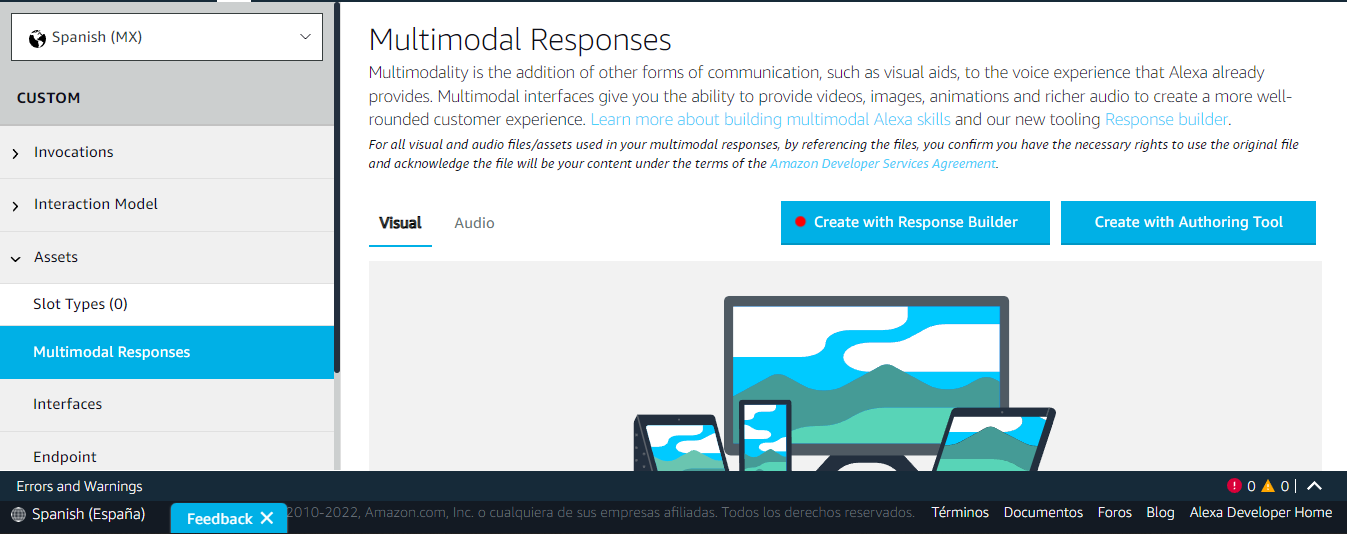
\includegraphics[width=0.70\textwidth]{Cap5/Figuras/AlexaMultimodalResponses.png}
  \caption{Interfaces con respuestas multimodales en la consola de desarrollo de Alexa.}
  \label{fig:51}
\end{figure}

La skill Buscador Gavilán, no es la excepción a la integración de interacción multimodal, en la que se pueden crear recursos visuales y táctiles. Es importante mencionar que la integración multimodal a una skill, está sujeta al diseño de una interfaz visual, por lo que sería necesario definir herramientas como el Customer Journey Map, un mapa de navegación, así como pruebas con usuarios para evaluar la usabilidad de la interfaz gráfica. Con el fin de limitar la skill Buscador Gavilán a una interacción basada únicamente en el reconocimiento por voz, la integración de interfaces multimodales se propone como trabajo a futuro para crear una mejor experiencia con la skill.

Algunos prototipos de la interacción multimodal con el Buscador Gavilán se presentan a continuación. Cabe destacar que estos sólo son prototipos de prueba para la integración multimodal, más no una versión final de los elementos visuales que presentan.

En la Figura \ref{fig:52} se muestra una propuesta para la bienvenida a la skill, una vez que es activado el LaunchRequestHandler a partir de uno de los comandos de activación de la skill.

\begin{figure}[H]
  \centering
  
\includegraphics[width=0.60\textwidth]{Cap5/Figuras/Multimodal1.png}
  \caption{Respuesta multimodal de bienvenida al Buscador Gavilán.}
  \label{fig:52}
\end{figure}

En la Figura \ref{fig:53} se muestra una propuesta para el listado de preguntas sugeridas para elegir una pregunta inicial.

\begin{figure}[H]
  \centering
  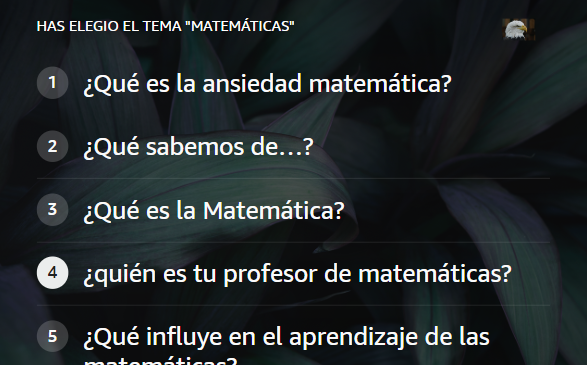
\includegraphics[width=0.60\textwidth]{Cap5/Figuras/Multimodal2.png}
  \caption{Respuesta multimodal para el listado de preguntas sugeridas del Buscador Gavilán.}
  \label{fig:53}
\end{figure}

En la Figura \ref{fig:54} se muestra una propuesta para el listado de fuentes de información con el dominio del cual se consulta la información.

\begin{figure}[H]
  \centering
  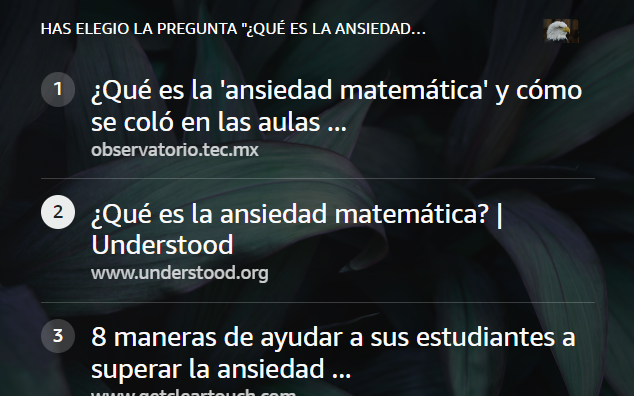
\includegraphics[width=0.60\textwidth]{Cap5/Figuras/Multimodal3.png}
  \caption{Respuesta multimodal para el listado de fuentes de información del Buscador Gavilán.}
  \label{fig:54}
\end{figure}

En la Figura \ref{fig:55} se muestra una propuesta para mostrar la información contenida en alguna de las fuentes de información elegida por el usuario.

\begin{figure}[H]
  \centering
  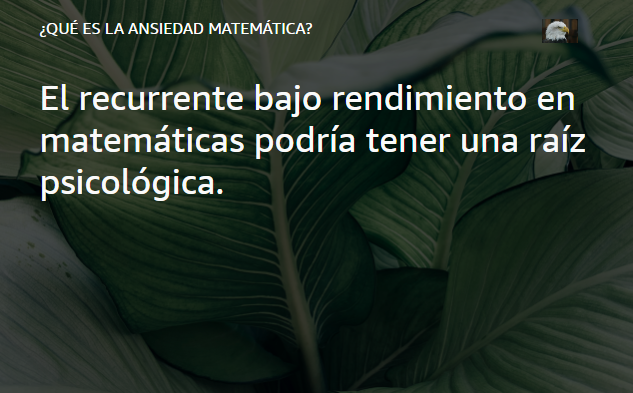
\includegraphics[width=0.60\textwidth]{Cap5/Figuras/Multimodal4.png}
  \caption{Respuesta multimodal para mostrar contenido de una fuente de información elegida.}
  \label{fig:55}
\end{figure}

En la Figura \ref{fig:56} se muestra una propuesta para mostrar al usuario las sugerencias generales para incorporar en la investigación final, así como brindarle la posibilidad de integrar un recordatorio.

\begin{figure}[H]
  \centering
  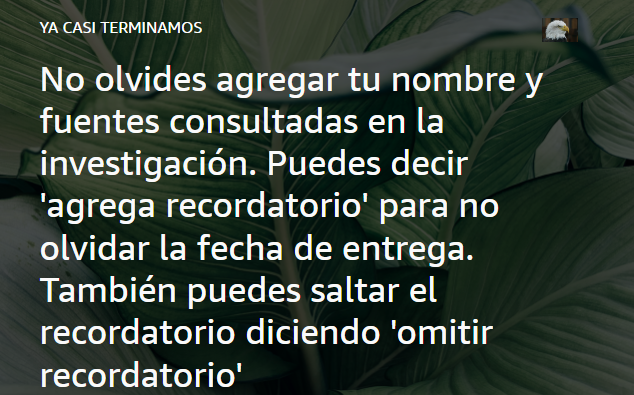
\includegraphics[width=0.60\textwidth]{Cap5/Figuras/Multimodal5.png}
  \caption{Respuesta multimodal para sugerir recomendaciones al usuario.}
  \label{fig:56}
\end{figure}

En la Figura \ref{fig:57} se muestra una propuesta para mostrar las recomendaciones para representar la información de la investigación final, así como la despedida de la skill.

\begin{figure}[H]
  \centering
  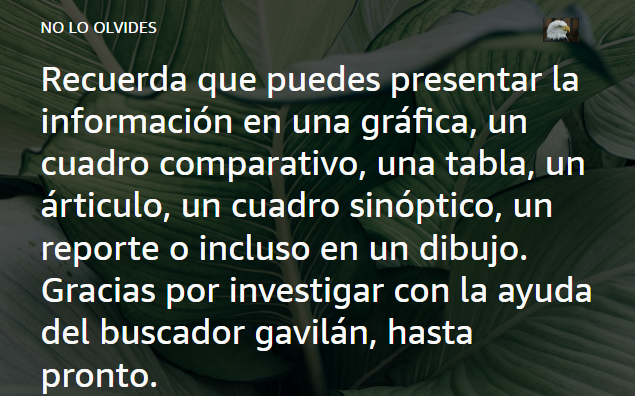
\includegraphics[width=0.60\textwidth]{Cap5/Figuras/Multimodal6.png}
  \caption{Respuesta multimodal para sugerir herramientas de representación de información.}
  \label{fig:57}
\end{figure}
